\documentclass[]{article}
\usepackage{lmodern}
\usepackage{amssymb,amsmath}
\usepackage{ifxetex,ifluatex}
\usepackage{fixltx2e} % provides \textsubscript
\ifnum 0\ifxetex 1\fi\ifluatex 1\fi=0 % if pdftex
  \usepackage[T1]{fontenc}
  \usepackage[utf8]{inputenc}
\else % if luatex or xelatex
  \ifxetex
    \usepackage{mathspec}
  \else
    \usepackage{fontspec}
  \fi
  \defaultfontfeatures{Ligatures=TeX,Scale=MatchLowercase}
\fi
% use upquote if available, for straight quotes in verbatim environments
\IfFileExists{upquote.sty}{\usepackage{upquote}}{}
% use microtype if available
\IfFileExists{microtype.sty}{%
\usepackage{microtype}
\UseMicrotypeSet[protrusion]{basicmath} % disable protrusion for tt fonts
}{}
\usepackage[margin=1in]{geometry}
\usepackage{hyperref}
\hypersetup{unicode=true,
            pdftitle={DATA 606 - Lab 7},
            pdfauthor={Joshua Sturm},
            pdfborder={0 0 0},
            breaklinks=true}
\urlstyle{same}  % don't use monospace font for urls
\usepackage{color}
\usepackage{fancyvrb}
\newcommand{\VerbBar}{|}
\newcommand{\VERB}{\Verb[commandchars=\\\{\}]}
\DefineVerbatimEnvironment{Highlighting}{Verbatim}{commandchars=\\\{\}}
% Add ',fontsize=\small' for more characters per line
\usepackage{framed}
\definecolor{shadecolor}{RGB}{248,248,248}
\newenvironment{Shaded}{\begin{snugshade}}{\end{snugshade}}
\newcommand{\KeywordTok}[1]{\textcolor[rgb]{0.13,0.29,0.53}{\textbf{#1}}}
\newcommand{\DataTypeTok}[1]{\textcolor[rgb]{0.13,0.29,0.53}{#1}}
\newcommand{\DecValTok}[1]{\textcolor[rgb]{0.00,0.00,0.81}{#1}}
\newcommand{\BaseNTok}[1]{\textcolor[rgb]{0.00,0.00,0.81}{#1}}
\newcommand{\FloatTok}[1]{\textcolor[rgb]{0.00,0.00,0.81}{#1}}
\newcommand{\ConstantTok}[1]{\textcolor[rgb]{0.00,0.00,0.00}{#1}}
\newcommand{\CharTok}[1]{\textcolor[rgb]{0.31,0.60,0.02}{#1}}
\newcommand{\SpecialCharTok}[1]{\textcolor[rgb]{0.00,0.00,0.00}{#1}}
\newcommand{\StringTok}[1]{\textcolor[rgb]{0.31,0.60,0.02}{#1}}
\newcommand{\VerbatimStringTok}[1]{\textcolor[rgb]{0.31,0.60,0.02}{#1}}
\newcommand{\SpecialStringTok}[1]{\textcolor[rgb]{0.31,0.60,0.02}{#1}}
\newcommand{\ImportTok}[1]{#1}
\newcommand{\CommentTok}[1]{\textcolor[rgb]{0.56,0.35,0.01}{\textit{#1}}}
\newcommand{\DocumentationTok}[1]{\textcolor[rgb]{0.56,0.35,0.01}{\textbf{\textit{#1}}}}
\newcommand{\AnnotationTok}[1]{\textcolor[rgb]{0.56,0.35,0.01}{\textbf{\textit{#1}}}}
\newcommand{\CommentVarTok}[1]{\textcolor[rgb]{0.56,0.35,0.01}{\textbf{\textit{#1}}}}
\newcommand{\OtherTok}[1]{\textcolor[rgb]{0.56,0.35,0.01}{#1}}
\newcommand{\FunctionTok}[1]{\textcolor[rgb]{0.00,0.00,0.00}{#1}}
\newcommand{\VariableTok}[1]{\textcolor[rgb]{0.00,0.00,0.00}{#1}}
\newcommand{\ControlFlowTok}[1]{\textcolor[rgb]{0.13,0.29,0.53}{\textbf{#1}}}
\newcommand{\OperatorTok}[1]{\textcolor[rgb]{0.81,0.36,0.00}{\textbf{#1}}}
\newcommand{\BuiltInTok}[1]{#1}
\newcommand{\ExtensionTok}[1]{#1}
\newcommand{\PreprocessorTok}[1]{\textcolor[rgb]{0.56,0.35,0.01}{\textit{#1}}}
\newcommand{\AttributeTok}[1]{\textcolor[rgb]{0.77,0.63,0.00}{#1}}
\newcommand{\RegionMarkerTok}[1]{#1}
\newcommand{\InformationTok}[1]{\textcolor[rgb]{0.56,0.35,0.01}{\textbf{\textit{#1}}}}
\newcommand{\WarningTok}[1]{\textcolor[rgb]{0.56,0.35,0.01}{\textbf{\textit{#1}}}}
\newcommand{\AlertTok}[1]{\textcolor[rgb]{0.94,0.16,0.16}{#1}}
\newcommand{\ErrorTok}[1]{\textcolor[rgb]{0.64,0.00,0.00}{\textbf{#1}}}
\newcommand{\NormalTok}[1]{#1}
\usepackage{graphicx,grffile}
\makeatletter
\def\maxwidth{\ifdim\Gin@nat@width>\linewidth\linewidth\else\Gin@nat@width\fi}
\def\maxheight{\ifdim\Gin@nat@height>\textheight\textheight\else\Gin@nat@height\fi}
\makeatother
% Scale images if necessary, so that they will not overflow the page
% margins by default, and it is still possible to overwrite the defaults
% using explicit options in \includegraphics[width, height, ...]{}
\setkeys{Gin}{width=\maxwidth,height=\maxheight,keepaspectratio}
\IfFileExists{parskip.sty}{%
\usepackage{parskip}
}{% else
\setlength{\parindent}{0pt}
\setlength{\parskip}{6pt plus 2pt minus 1pt}
}
\setlength{\emergencystretch}{3em}  % prevent overfull lines
\providecommand{\tightlist}{%
  \setlength{\itemsep}{0pt}\setlength{\parskip}{0pt}}
\setcounter{secnumdepth}{0}
% Redefines (sub)paragraphs to behave more like sections
\ifx\paragraph\undefined\else
\let\oldparagraph\paragraph
\renewcommand{\paragraph}[1]{\oldparagraph{#1}\mbox{}}
\fi
\ifx\subparagraph\undefined\else
\let\oldsubparagraph\subparagraph
\renewcommand{\subparagraph}[1]{\oldsubparagraph{#1}\mbox{}}
\fi

%%% Use protect on footnotes to avoid problems with footnotes in titles
\let\rmarkdownfootnote\footnote%
\def\footnote{\protect\rmarkdownfootnote}

%%% Change title format to be more compact
\usepackage{titling}

% Create subtitle command for use in maketitle
\newcommand{\subtitle}[1]{
  \posttitle{
    \begin{center}\large#1\end{center}
    }
}

\setlength{\droptitle}{-2em}
  \title{DATA 606 - Lab 7}
  \pretitle{\vspace{\droptitle}\centering\huge}
  \posttitle{\par}
  \author{Joshua Sturm}
  \preauthor{\centering\large\emph}
  \postauthor{\par}
  \date{}
  \predate{}\postdate{}


\begin{document}
\maketitle

\begin{Shaded}
\begin{Highlighting}[]
\KeywordTok{library}\NormalTok{(tidyverse)}
\KeywordTok{library}\NormalTok{(ggplot2)}
\end{Highlighting}
\end{Shaded}

\subsection{Batter up}\label{batter-up}

The movie
\href{http://en.wikipedia.org/wiki/Moneyball_(film)}{Moneyball} focuses
on the ``quest for the secret of success in baseball''. It follows a
low-budget team, the Oakland Athletics, who believed that underused
statistics, such as a player's ability to get on base, better predict
the ability to score runs than typical statistics like home runs, RBIs
(runs batted in), and batting average. Obtaining players who excelled in
these underused statistics turned out to be much more affordable for the
team.

In this lab we'll be looking at data from all 30 Major League Baseball
teams and examining the linear relationship between runs scored in a
season and a number of other player statistics. Our aim will be to
summarize these relationships both graphically and numerically in order
to find which variable, if any, helps us best predict a team's runs
scored in a season.

\subsection{The data}\label{the-data}

Let's load up the data for the 2011 season.

\begin{Shaded}
\begin{Highlighting}[]
\KeywordTok{load}\NormalTok{(}\StringTok{"more/mlb11.RData"}\NormalTok{)}
\end{Highlighting}
\end{Shaded}

In addition to runs scored, there are seven traditionally used variables
in the data set: at-bats, hits, home runs, batting average, strikeouts,
stolen bases, and wins. There are also three newer variables: on-base
percentage, slugging percentage, and on-base plus slugging. For the
first portion of the analysis we'll consider the seven traditional
variables. At the end of the lab, you'll work with the newer variables
on your own.

\subsection{Question 1}\label{question-1}

What type of plot would you use to display the relationship between
\texttt{runs} and one of the other numerical variables? Plot this
relationship using the variable \texttt{at\_bats} as the predictor. Does
the relationship look linear? If you knew a team's \texttt{at\_bats},
would you be comfortable using a linear model to predict the number of
runs?

\subsubsection{Solution}\label{solution}

We can use a scatter plot to look for any relationships.

\begin{Shaded}
\begin{Highlighting}[]
\KeywordTok{ggplot}\NormalTok{(mlb11, }\KeywordTok{aes}\NormalTok{(}\DataTypeTok{x=}\NormalTok{at_bats, }\DataTypeTok{y=}\NormalTok{runs)) }\OperatorTok{+}
\StringTok{  }\KeywordTok{geom_point}\NormalTok{(}\DataTypeTok{colour=}\StringTok{"green"}\NormalTok{)}
\end{Highlighting}
\end{Shaded}

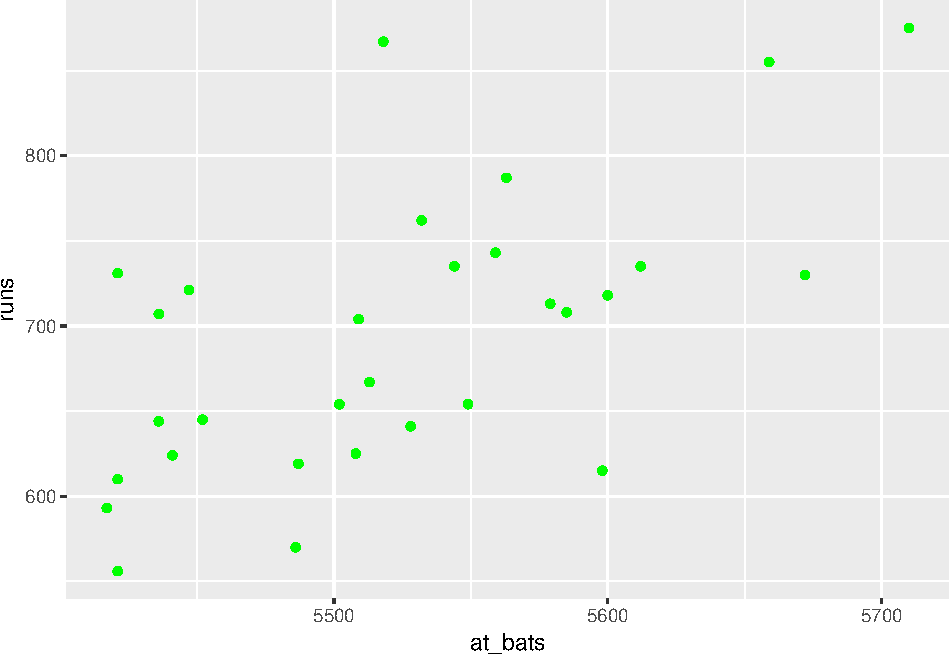
\includegraphics{DATA_606_Lab_7_files/figure-latex/quest-one-plot-1.pdf}
Based on the scatter plot, the relationship between \texttt{at\_bats}
and \texttt{runs} does appear to be linear, and I would use a linear
model to predict the number of runs.

If the relationship looks linear, we can quantify the strength of the
relationship with the correlation coefficient.

\begin{Shaded}
\begin{Highlighting}[]
\KeywordTok{cor}\NormalTok{(mlb11}\OperatorTok{$}\NormalTok{runs, mlb11}\OperatorTok{$}\NormalTok{at_bats)}
\end{Highlighting}
\end{Shaded}

\begin{verbatim}
## [1] 0.610627
\end{verbatim}

\subsection{Sum of squared residuals}\label{sum-of-squared-residuals}

Think back to the way that we described the distribution of a single
variable. Recall that we discussed characteristics such as center,
spread, and shape. It's also useful to be able to describe the
relationship of two numerical variables, such as \texttt{runs} and
\texttt{at\_bats} above.

\subsection{Question 2}\label{question-2}

Looking at your plot from the previous exercise, describe the
relationship between these two variables. Make sure to discuss the form,
direction, and strength of the relationship as well as any unusual
observations.

\subsubsection{Solution}\label{solution-1}

There is a positive correlation between number of at bats and number of
runs, with a few outliers.

Just as we used the mean and standard deviation to summarize a single
variable, we can summarize the relationship between these two variables
by finding the line that best follows their association. Use the
following interactive function to select the line that you think does
the best job of going through the cloud of points.

\begin{Shaded}
\begin{Highlighting}[]
\KeywordTok{plot_ss}\NormalTok{(}\DataTypeTok{x =}\NormalTok{ mlb11}\OperatorTok{$}\NormalTok{at_bats, }\DataTypeTok{y =}\NormalTok{ mlb11}\OperatorTok{$}\NormalTok{runs)}
\end{Highlighting}
\end{Shaded}

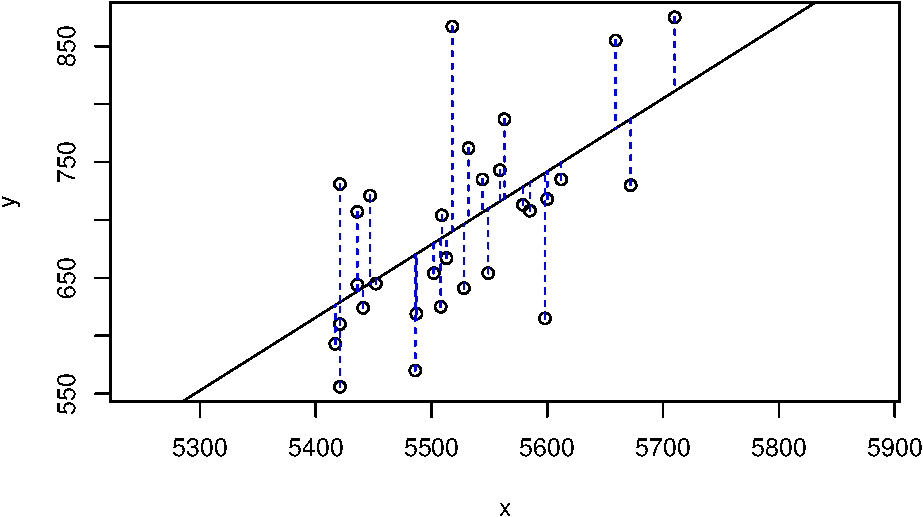
\includegraphics{DATA_606_Lab_7_files/figure-latex/plotss-atbats-runs-1.pdf}

\begin{verbatim}
## Click two points to make a line.
                                
## Call:
## lm(formula = y ~ x, data = pts)
## 
## Coefficients:
## (Intercept)            x  
##  -2789.2429       0.6305  
## 
## Sum of Squares:  123721.9
\end{verbatim}

After running this command, you'll be prompted to click two points on
the plot to define a line. Once you've done that, the line you specified
will be shown in black and the residuals in blue. Note that there are 30
residuals, one for each of the 30 observations. Recall that the
residuals are the difference between the observed values and the values
predicted by the line:

\[
  e_i = y_i - \hat{y}_i
\]

The most common way to do linear regression is to select the line that
minimizes the sum of squared residuals. To visualize the squared
residuals, you can rerun the plot command and add the argument
\texttt{showSquares\ =\ TRUE}.

\begin{Shaded}
\begin{Highlighting}[]
\KeywordTok{plot_ss}\NormalTok{(}\DataTypeTok{x =}\NormalTok{ mlb11}\OperatorTok{$}\NormalTok{at_bats, }\DataTypeTok{y =}\NormalTok{ mlb11}\OperatorTok{$}\NormalTok{runs, }\DataTypeTok{showSquares =} \OtherTok{TRUE}\NormalTok{)}
\end{Highlighting}
\end{Shaded}

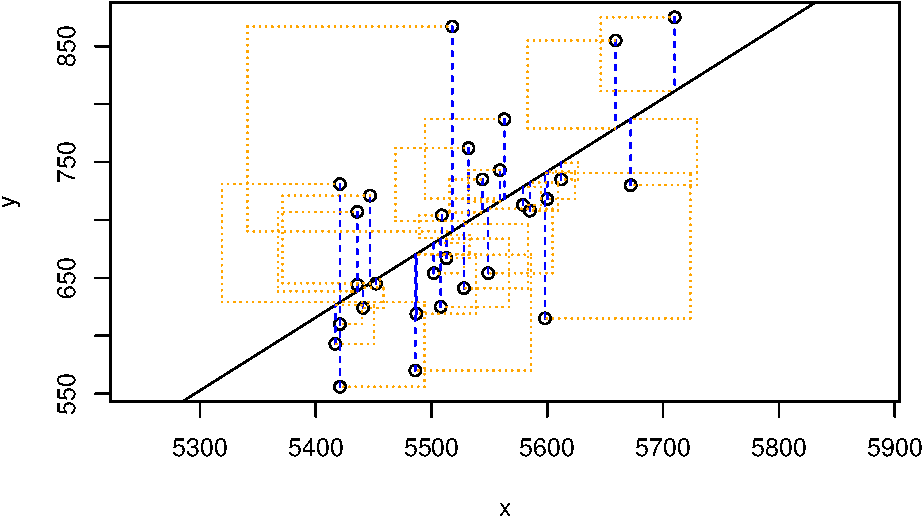
\includegraphics{DATA_606_Lab_7_files/figure-latex/plotss-atbats-runs-squares-1.pdf}

\begin{verbatim}
## Click two points to make a line.
                                
## Call:
## lm(formula = y ~ x, data = pts)
## 
## Coefficients:
## (Intercept)            x  
##  -2789.2429       0.6305  
## 
## Sum of Squares:  123721.9
\end{verbatim}

Note that the output from the \texttt{plot\_ss} function provides you
with the slope and intercept of your line as well as the sum of squares.

\subsection{Question 3}\label{question-3}

Using \texttt{plot\_ss}, choose a line that does a good job of
minimizing the sum of squares. Run the function several times. What was
the smallest sum of squares that you got? How does it compare to your
neighbors?

\subsubsection{Solution}\label{solution-2}

The lowest of 5 runs was 125590.4.

\subsection{The linear model}\label{the-linear-model}

It is rather cumbersome to try to get the correct least squares line,
i.e.~the line that minimizes the sum of squared residuals, through trial
and error. Instead we can use the \texttt{lm} function in R to fit the
linear model (a.k.a. regression line).

\begin{Shaded}
\begin{Highlighting}[]
\NormalTok{m1 <-}\StringTok{ }\KeywordTok{lm}\NormalTok{(runs }\OperatorTok{~}\StringTok{ }\NormalTok{at_bats, }\DataTypeTok{data =}\NormalTok{ mlb11)}
\end{Highlighting}
\end{Shaded}

The first argument in the function \texttt{lm} is a formula that takes
the form \texttt{y\ \textasciitilde{}\ x}. Here it can be read that we
want to make a linear model of \texttt{runs} as a function of
\texttt{at\_bats}. The second argument specifies that R should look in
the \texttt{mlb11} data frame to find the \texttt{runs} and
\texttt{at\_bats} variables.

The output of \texttt{lm} is an object that contains all of the
information we need about the linear model that was just fit. We can
access this information using the summary function.

\begin{Shaded}
\begin{Highlighting}[]
\KeywordTok{summary}\NormalTok{(m1)}
\end{Highlighting}
\end{Shaded}

\begin{verbatim}
## 
## Call:
## lm(formula = runs ~ at_bats, data = mlb11)
## 
## Residuals:
##     Min      1Q  Median      3Q     Max 
## -125.58  -47.05  -16.59   54.40  176.87 
## 
## Coefficients:
##               Estimate Std. Error t value Pr(>|t|)    
## (Intercept) -2789.2429   853.6957  -3.267 0.002871 ** 
## at_bats         0.6305     0.1545   4.080 0.000339 ***
## ---
## Signif. codes:  0 '***' 0.001 '**' 0.01 '*' 0.05 '.' 0.1 ' ' 1
## 
## Residual standard error: 66.47 on 28 degrees of freedom
## Multiple R-squared:  0.3729, Adjusted R-squared:  0.3505 
## F-statistic: 16.65 on 1 and 28 DF,  p-value: 0.0003388
\end{verbatim}

Let's consider this output piece by piece. First, the formula used to
describe the model is shown at the top. After the formula you find the
five-number summary of the residuals. The ``Coefficients'' table shown
next is key; its first column displays the linear model's y-intercept
and the coefficient of \texttt{at\_bats}. With this table, we can write
down the least squares regression line for the linear model:

\[
  \hat{y} = -2789.2429 + 0.6305 * atbats
\]

One last piece of information we will discuss from the summary output is
the Multiple R-squared, or more simply, \(R^2\). The \(R^2\) value
represents the proportion of variability in the response variable that
is explained by the explanatory variable. For this model, 37.3\% of the
variability in runs is explained by at-bats.

\subsection{Question 4}\label{question-4}

Fit a new model that uses \texttt{homeruns} to predict \texttt{runs}.
Using the estimates from the R output, write the equation of the
regression line. What does the slope tell us in the context of the
relationship between success of a team and its home runs?

\subsubsection{Solution}\label{solution-3}

\begin{Shaded}
\begin{Highlighting}[]
\KeywordTok{plot_ss}\NormalTok{(}\DataTypeTok{x =}\NormalTok{ mlb11}\OperatorTok{$}\NormalTok{homeruns, }\DataTypeTok{y =}\NormalTok{ mlb11}\OperatorTok{$}\NormalTok{runs, }\DataTypeTok{showSquares =} \OtherTok{TRUE}\NormalTok{)}
\end{Highlighting}
\end{Shaded}

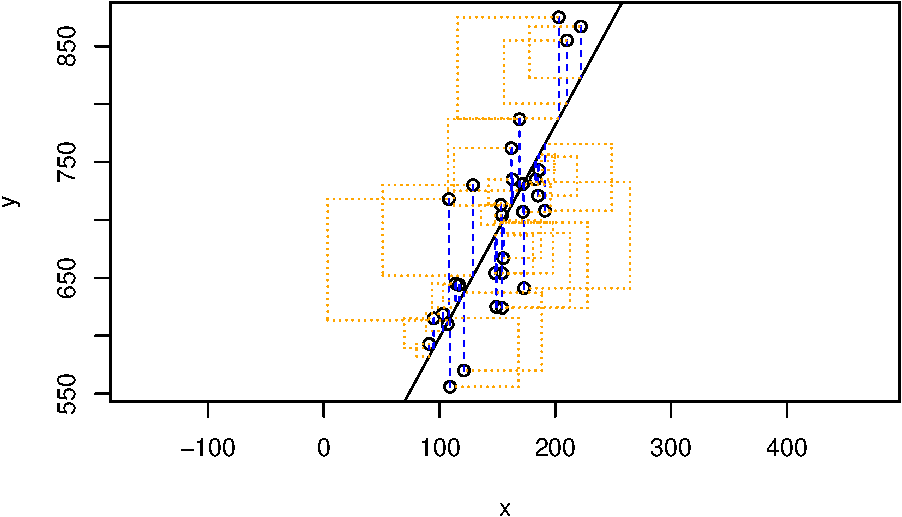
\includegraphics{DATA_606_Lab_7_files/figure-latex/unnamed-chunk-1-1.pdf}

\begin{verbatim}
## Click two points to make a line.
                                
## Call:
## lm(formula = y ~ x, data = pts)
## 
## Coefficients:
## (Intercept)            x  
##     415.239        1.835  
## 
## Sum of Squares:  73671.99
\end{verbatim}

\begin{Shaded}
\begin{Highlighting}[]
\KeywordTok{cor}\NormalTok{(mlb11}\OperatorTok{$}\NormalTok{runs, mlb11}\OperatorTok{$}\NormalTok{homeruns)}
\end{Highlighting}
\end{Shaded}

\begin{verbatim}
## [1] 0.7915577
\end{verbatim}

\begin{Shaded}
\begin{Highlighting}[]
\NormalTok{m2 <-}\StringTok{ }\KeywordTok{lm}\NormalTok{(runs }\OperatorTok{~}\StringTok{ }\NormalTok{homeruns, }\DataTypeTok{data =}\NormalTok{ mlb11)}
\KeywordTok{summary}\NormalTok{(m2)}
\end{Highlighting}
\end{Shaded}

\begin{verbatim}
## 
## Call:
## lm(formula = runs ~ homeruns, data = mlb11)
## 
## Residuals:
##     Min      1Q  Median      3Q     Max 
## -91.615 -33.410   3.231  24.292 104.631 
## 
## Coefficients:
##             Estimate Std. Error t value Pr(>|t|)    
## (Intercept) 415.2389    41.6779   9.963 1.04e-10 ***
## homeruns      1.8345     0.2677   6.854 1.90e-07 ***
## ---
## Signif. codes:  0 '***' 0.001 '**' 0.01 '*' 0.05 '.' 0.1 ' ' 1
## 
## Residual standard error: 51.29 on 28 degrees of freedom
## Multiple R-squared:  0.6266, Adjusted R-squared:  0.6132 
## F-statistic: 46.98 on 1 and 28 DF,  p-value: 1.9e-07
\end{verbatim}

The equation for the regression line is
\(\hat{y} = 415.2389 + 1.8345 * \text{homeruns}\). There is a strong
correlation between homeruns and number of runs; the more homeruns, the
more runs.

\subsection{Prediction and prediction
errors}\label{prediction-and-prediction-errors}

Let's create a scatterplot with the least squares line laid on top.

\begin{Shaded}
\begin{Highlighting}[]
\KeywordTok{plot}\NormalTok{(mlb11}\OperatorTok{$}\NormalTok{runs }\OperatorTok{~}\StringTok{ }\NormalTok{mlb11}\OperatorTok{$}\NormalTok{at_bats)}
\KeywordTok{abline}\NormalTok{(m1)}
\end{Highlighting}
\end{Shaded}

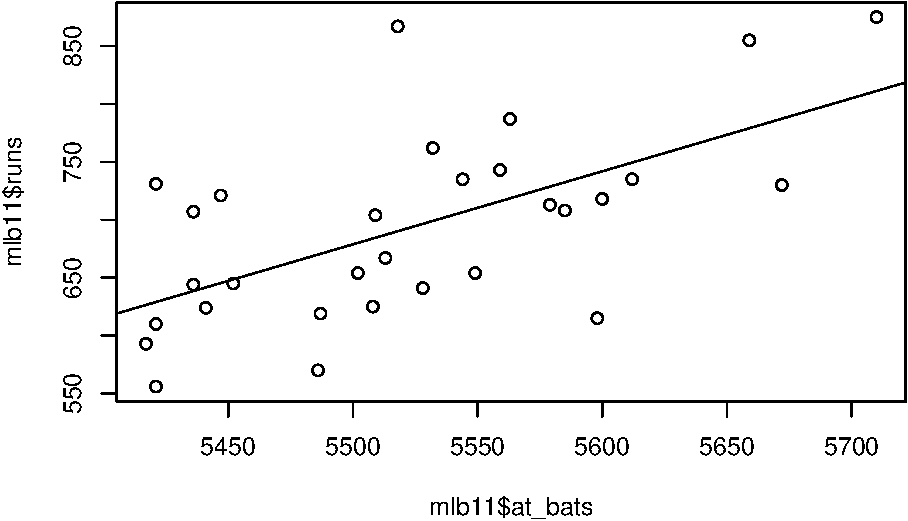
\includegraphics{DATA_606_Lab_7_files/figure-latex/reg-with-line-1.pdf}

The function \texttt{abline} plots a line based on its slope and
intercept. Here, we used a shortcut by providing the model \texttt{m1},
which contains both parameter estimates. This line can be used to
predict \(y\) at any value of \(x\). When predictions are made for
values of \(x\) that are beyond the range of the observed data, it is
referred to as \emph{extrapolation} and is not usually recommended.
However, predictions made within the range of the data are more
reliable. They're also used to compute the residuals.

\subsection{Question 5}\label{question-5}

If a team manager saw the least squares regression line and not the
actual data, how many runs would he or she predict for a team with 5,578
at-bats? Is this an overestimate or an underestimate, and by how much?
In other words, what is the residual for this prediction?

\subsubsection{Solution}\label{solution-4}

\begin{Shaded}
\begin{Highlighting}[]
\NormalTok{runs.prediction <-}\StringTok{ }\NormalTok{m1}\OperatorTok{$}\NormalTok{coefficients[[}\DecValTok{1}\NormalTok{]] }\OperatorTok{+}\StringTok{ }\NormalTok{(m1}\OperatorTok{$}\NormalTok{coefficients[[}\DecValTok{2}\NormalTok{]] }\OperatorTok{*}\StringTok{ }\DecValTok{5578}\NormalTok{)}
\KeywordTok{round}\NormalTok{(runs.prediction, }\DecValTok{1}\NormalTok{)}
\end{Highlighting}
\end{Shaded}

\begin{verbatim}
## [1] 728
\end{verbatim}

\begin{Shaded}
\begin{Highlighting}[]
\NormalTok{runs.residual <-}\StringTok{ }\NormalTok{mlb11}\OperatorTok{$}\NormalTok{runs[mlb11}\OperatorTok{$}\NormalTok{at_bats }\OperatorTok{==}\StringTok{ }\DecValTok{5579}\NormalTok{] }\OperatorTok{-}\StringTok{ }\NormalTok{runs.prediction}
\KeywordTok{round}\NormalTok{(runs.residual,}\DecValTok{1}\NormalTok{)}
\end{Highlighting}
\end{Shaded}

\begin{verbatim}
## [1] -15
\end{verbatim}

The manager overpredicted, with a residual of -14.9649746.

\subsection{Model diagnostics}\label{model-diagnostics}

To assess whether the linear model is reliable, we need to check for (1)
linearity, (2) nearly normal residuals, and (3) constant variability.

\emph{Linearity}: You already checked if the relationship between runs
and at-bats is linear using a scatterplot. We should also verify this
condition with a plot of the residuals vs.~at-bats. Recall that any code
following a \emph{\#} is intended to be a comment that helps understand
the code but is ignored by R.

\begin{Shaded}
\begin{Highlighting}[]
\KeywordTok{plot}\NormalTok{(m1}\OperatorTok{$}\NormalTok{residuals }\OperatorTok{~}\StringTok{ }\NormalTok{mlb11}\OperatorTok{$}\NormalTok{at_bats)}
\KeywordTok{abline}\NormalTok{(}\DataTypeTok{h =} \DecValTok{0}\NormalTok{, }\DataTypeTok{lty =} \DecValTok{3}\NormalTok{)  }\CommentTok{# adds a horizontal dashed line at y = 0}
\end{Highlighting}
\end{Shaded}

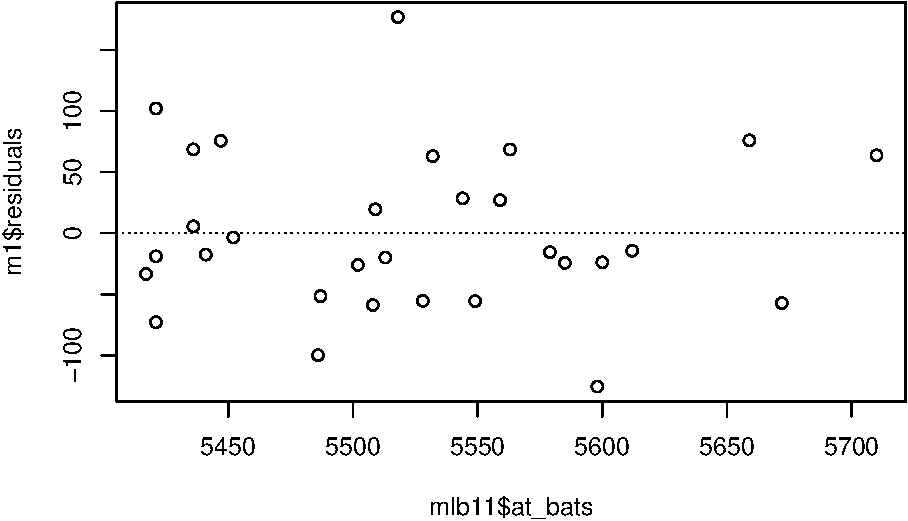
\includegraphics{DATA_606_Lab_7_files/figure-latex/residuals-1.pdf}

\subsection{Question 6}\label{question-6}

Is there any apparent pattern in the residuals plot? What does this
indicate about the linearity of the relationship between runs and
at-bats?

\subsubsection{Solution}\label{solution-5}

There is no apparent pattern, and the residuals are centered around the
center (0), which would imply a linear relationship.

\emph{Nearly normal residuals}: To check this condition, we can look at
a histogram

\begin{Shaded}
\begin{Highlighting}[]
\KeywordTok{hist}\NormalTok{(m1}\OperatorTok{$}\NormalTok{residuals)}
\end{Highlighting}
\end{Shaded}

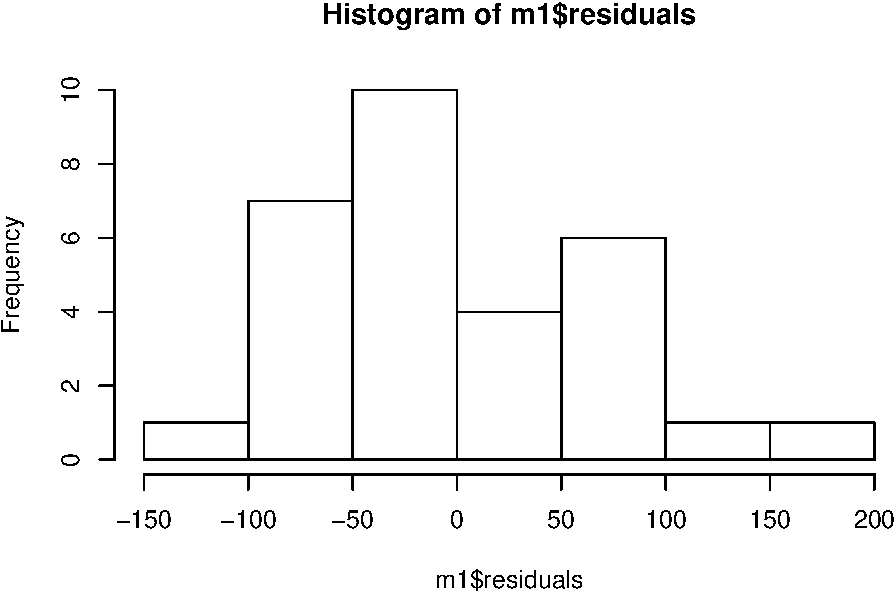
\includegraphics{DATA_606_Lab_7_files/figure-latex/hist-res-1.pdf}

or a normal probability plot of the residuals.

\begin{Shaded}
\begin{Highlighting}[]
\KeywordTok{qqnorm}\NormalTok{(m1}\OperatorTok{$}\NormalTok{residuals)}
\KeywordTok{qqline}\NormalTok{(m1}\OperatorTok{$}\NormalTok{residuals)  }\CommentTok{# adds diagonal line to the normal prob plot}
\end{Highlighting}
\end{Shaded}

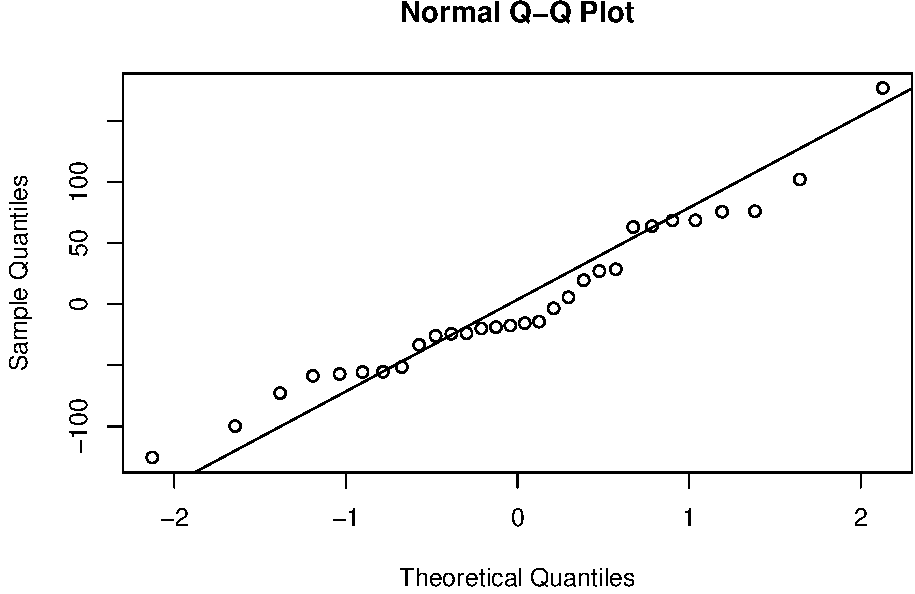
\includegraphics{DATA_606_Lab_7_files/figure-latex/qq-res-1.pdf}

\subsection{Question 7}\label{question-7}

Based on the histogram and the normal probability plot, does the nearly
normal residuals condition appear to be met?

\subsubsection{Solution}\label{solution-6}

Both plots have a slight skew, but there are enough samples to assume
nearly normal.

\emph{Constant variability}:

\subsection{Question 8}\label{question-8}

Based on the plot in (1), does the constant variability condition appear
to be met?

\subsubsection{Solution}\label{solution-7}

Yes, the points don't stray far from the least squares line.

\begin{center}\rule{0.5\linewidth}{\linethickness}\end{center}

\subsection{On Your Own}\label{on-your-own}

\subsection{Question 9}\label{question-9}

Choose another traditional variable from \texttt{mlb11} that you think
might be a good predictor of \texttt{runs}. Produce a scatterplot of the
two variables and fit a linear model. At a glance, does there seem to be
a linear relationship?

\subsubsection{Solution}\label{solution-8}

We'll use the variable \texttt{hits}; the more hits, statisticall, there
should be more runs.

\begin{Shaded}
\begin{Highlighting}[]
\KeywordTok{ggplot}\NormalTok{(mlb11, }\KeywordTok{aes}\NormalTok{(}\DataTypeTok{x=}\NormalTok{hits, }\DataTypeTok{y=}\NormalTok{runs)) }\OperatorTok{+}
\StringTok{  }\KeywordTok{geom_point}\NormalTok{(}\DataTypeTok{colour =} \StringTok{'green'}\NormalTok{) }\OperatorTok{+}
\StringTok{  }\KeywordTok{geom_smooth}\NormalTok{(}\DataTypeTok{method =} \StringTok{'lm'}\NormalTok{)}
\end{Highlighting}
\end{Shaded}

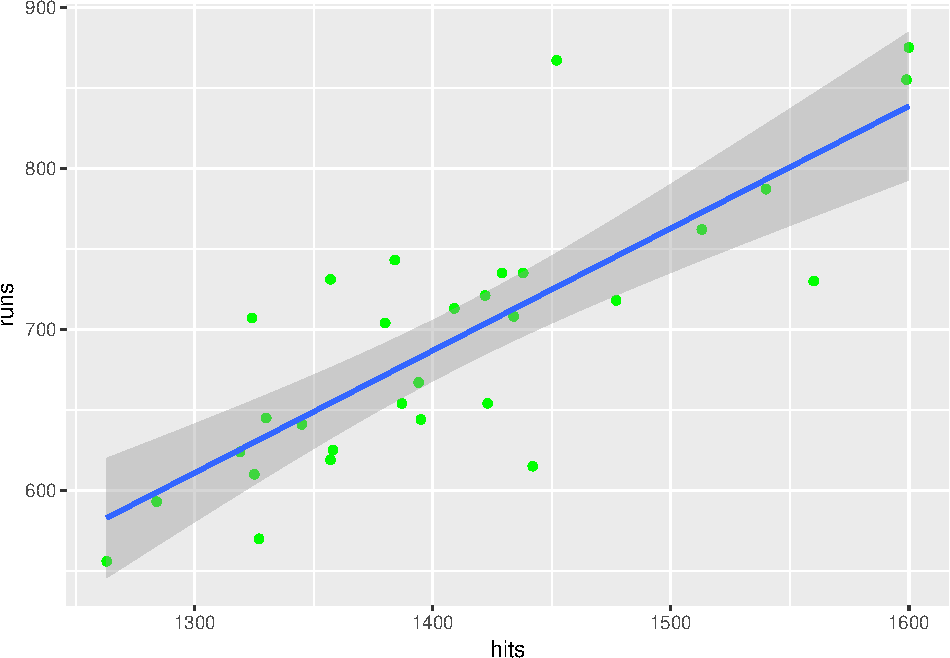
\includegraphics{DATA_606_Lab_7_files/figure-latex/question-nine-1.pdf}
There does appear to be a linear relationship.

\subsection{Question 10}\label{question-10}

How does this relationship compare to the relationship between
\texttt{runs} and \texttt{at\_bats}? Use the R\(^2\) values from the two
model summaries to compare. Does your variable seem to predict
\texttt{runs} better than \texttt{at\_bats}? How can you tell?

\subsubsection{Solution}\label{solution-9}

\begin{Shaded}
\begin{Highlighting}[]
\NormalTok{m3 <-}\StringTok{ }\KeywordTok{lm}\NormalTok{(runs }\OperatorTok{~}\StringTok{ }\NormalTok{hits, }\DataTypeTok{data=}\NormalTok{mlb11)}
\KeywordTok{summary}\NormalTok{(m1)}
\end{Highlighting}
\end{Shaded}

\begin{verbatim}
## 
## Call:
## lm(formula = runs ~ at_bats, data = mlb11)
## 
## Residuals:
##     Min      1Q  Median      3Q     Max 
## -125.58  -47.05  -16.59   54.40  176.87 
## 
## Coefficients:
##               Estimate Std. Error t value Pr(>|t|)    
## (Intercept) -2789.2429   853.6957  -3.267 0.002871 ** 
## at_bats         0.6305     0.1545   4.080 0.000339 ***
## ---
## Signif. codes:  0 '***' 0.001 '**' 0.01 '*' 0.05 '.' 0.1 ' ' 1
## 
## Residual standard error: 66.47 on 28 degrees of freedom
## Multiple R-squared:  0.3729, Adjusted R-squared:  0.3505 
## F-statistic: 16.65 on 1 and 28 DF,  p-value: 0.0003388
\end{verbatim}

\begin{Shaded}
\begin{Highlighting}[]
\KeywordTok{summary}\NormalTok{(m3)}
\end{Highlighting}
\end{Shaded}

\begin{verbatim}
## 
## Call:
## lm(formula = runs ~ hits, data = mlb11)
## 
## Residuals:
##      Min       1Q   Median       3Q      Max 
## -103.718  -27.179   -5.233   19.322  140.693 
## 
## Coefficients:
##              Estimate Std. Error t value Pr(>|t|)    
## (Intercept) -375.5600   151.1806  -2.484   0.0192 *  
## hits           0.7589     0.1071   7.085 1.04e-07 ***
## ---
## Signif. codes:  0 '***' 0.001 '**' 0.01 '*' 0.05 '.' 0.1 ' ' 1
## 
## Residual standard error: 50.23 on 28 degrees of freedom
## Multiple R-squared:  0.6419, Adjusted R-squared:  0.6292 
## F-statistic:  50.2 on 1 and 28 DF,  p-value: 1.043e-07
\end{verbatim}

The \(R^2\) for \texttt{at\_bats} is 0.3729, while the \(R^2\) for
\texttt{hits} is 0.6419, which tells us that \texttt{hits} is a better
predictor of runs than \texttt{at\_bats}.

\subsection{Question 11}\label{question-11}

Now that you can summarize the linear relationship between two
variables, investigate the relationships between \texttt{runs} and each
of the other five traditional variables. Which variable best predicts
\texttt{runs}? Support your conclusion using the graphical and numerical
methods we've discussed (for the sake of conciseness, only include
output for the best variable, not all five).

\subsubsection{Solution}\label{solution-10}

\begin{Shaded}
\begin{Highlighting}[]
\NormalTok{m4 <-}\StringTok{ }\KeywordTok{lm}\NormalTok{(runs }\OperatorTok{~}\StringTok{ }\NormalTok{bat_avg, }\DataTypeTok{data =}\NormalTok{ mlb11)}
\NormalTok{m5 <-}\StringTok{ }\KeywordTok{lm}\NormalTok{(runs }\OperatorTok{~}\StringTok{ }\NormalTok{strikeouts, }\DataTypeTok{data =}\NormalTok{ mlb11)}
\NormalTok{m6 <-}\StringTok{ }\KeywordTok{lm}\NormalTok{(runs }\OperatorTok{~}\StringTok{ }\NormalTok{stolen_bases, }\DataTypeTok{data =}\NormalTok{ mlb11)}
\NormalTok{m7 <-}\StringTok{ }\KeywordTok{lm}\NormalTok{(runs }\OperatorTok{~}\StringTok{ }\NormalTok{wins, }\DataTypeTok{data =}\NormalTok{ mlb11)}

\NormalTok{m <-}\StringTok{ }\KeywordTok{c}\NormalTok{(}\StringTok{'m1'}\NormalTok{, }\StringTok{'m2'}\NormalTok{, }\StringTok{'m3'}\NormalTok{, }\StringTok{'m4'}\NormalTok{, }\StringTok{'m5'}\NormalTok{, }\StringTok{'m6'}\NormalTok{, }\StringTok{'m7'}\NormalTok{)}
\NormalTok{r.squared <-}\StringTok{ }\KeywordTok{c}\NormalTok{(}\KeywordTok{summary}\NormalTok{(m1)[[}\DecValTok{8}\NormalTok{]], }\KeywordTok{summary}\NormalTok{(m2)[[}\DecValTok{8}\NormalTok{]], }\KeywordTok{summary}\NormalTok{(m3)[[}\DecValTok{8}\NormalTok{]], }\KeywordTok{summary}\NormalTok{(m4)[[}\DecValTok{8}\NormalTok{]], }\KeywordTok{summary}\NormalTok{(m5)[[}\DecValTok{8}\NormalTok{]], }\KeywordTok{summary}\NormalTok{(m6)[[}\DecValTok{8}\NormalTok{]], }\KeywordTok{summary}\NormalTok{(m7)[[}\DecValTok{8}\NormalTok{]])}

\NormalTok{mdf <-}\StringTok{ }\KeywordTok{data.frame}\NormalTok{(m, r.squared)}
\NormalTok{mdf}
\end{Highlighting}
\end{Shaded}

\begin{verbatim}
##    m   r.squared
## 1 m1 0.372865390
## 2 m2 0.626563570
## 3 m3 0.641938767
## 4 m4 0.656077135
## 5 m5 0.169357932
## 6 m6 0.002913993
## 7 m7 0.360971179
\end{verbatim}

\textasciitilde{}, runs, bat\_avg: \texttt{bat\_avg} is the best
predictor for the number of \texttt{runs}.

\subsection{Question 12}\label{question-12}

Now examine the three newer variables. These are the statistics used by
the author of \emph{Moneyball} to predict a teams success. In general,
are they more or less effective at predicting runs that the old
variables? Explain using appropriate graphical and numerical evidence.
Of all ten variables we've analyzed, which seems to be the best
predictor of \texttt{runs}? Using the limited (or not so limited)
information you know about these baseball statistics, does your result
make sense?

\subsubsection{Solution}\label{solution-11}

\begin{Shaded}
\begin{Highlighting}[]
\NormalTok{m8 <-}\StringTok{ }\KeywordTok{lm}\NormalTok{(runs }\OperatorTok{~}\StringTok{ }\NormalTok{new_onbase, }\DataTypeTok{data =}\NormalTok{ mlb11)}
\NormalTok{m9 <-}\StringTok{ }\KeywordTok{lm}\NormalTok{(runs }\OperatorTok{~}\StringTok{ }\NormalTok{new_slug, }\DataTypeTok{data =}\NormalTok{ mlb11)}
\NormalTok{m10 <-}\StringTok{ }\KeywordTok{lm}\NormalTok{(runs }\OperatorTok{~}\StringTok{ }\NormalTok{new_obs, }\DataTypeTok{data =}\NormalTok{ mlb11)}

\KeywordTok{ggplot}\NormalTok{(mlb11, }\KeywordTok{aes}\NormalTok{(}\DataTypeTok{x=}\NormalTok{new_onbase, }\DataTypeTok{y=}\NormalTok{runs)) }\OperatorTok{+}
\StringTok{  }\KeywordTok{geom_point}\NormalTok{(}\DataTypeTok{colour =} \StringTok{'green'}\NormalTok{) }\OperatorTok{+}
\StringTok{  }\KeywordTok{geom_smooth}\NormalTok{(}\DataTypeTok{method =} \StringTok{'lm'}\NormalTok{)}
\end{Highlighting}
\end{Shaded}

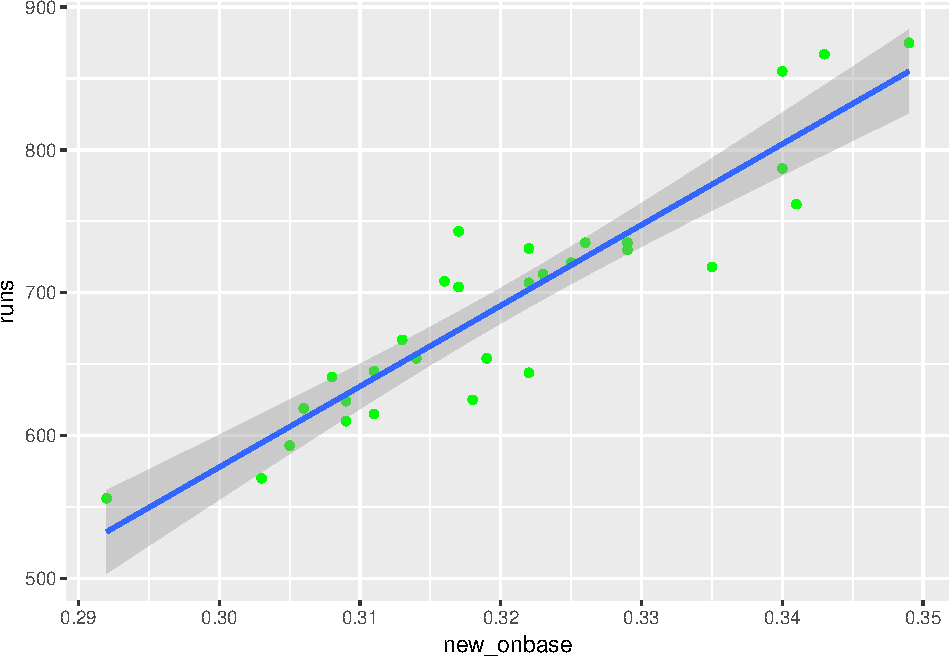
\includegraphics{DATA_606_Lab_7_files/figure-latex/unnamed-chunk-3-1.pdf}

\begin{Shaded}
\begin{Highlighting}[]
\KeywordTok{ggplot}\NormalTok{(mlb11, }\KeywordTok{aes}\NormalTok{(}\DataTypeTok{x=}\NormalTok{new_slug, }\DataTypeTok{y=}\NormalTok{runs)) }\OperatorTok{+}
\StringTok{  }\KeywordTok{geom_point}\NormalTok{(}\DataTypeTok{colour =} \StringTok{'green'}\NormalTok{) }\OperatorTok{+}
\StringTok{  }\KeywordTok{geom_smooth}\NormalTok{(}\DataTypeTok{method =} \StringTok{'lm'}\NormalTok{)}
\end{Highlighting}
\end{Shaded}

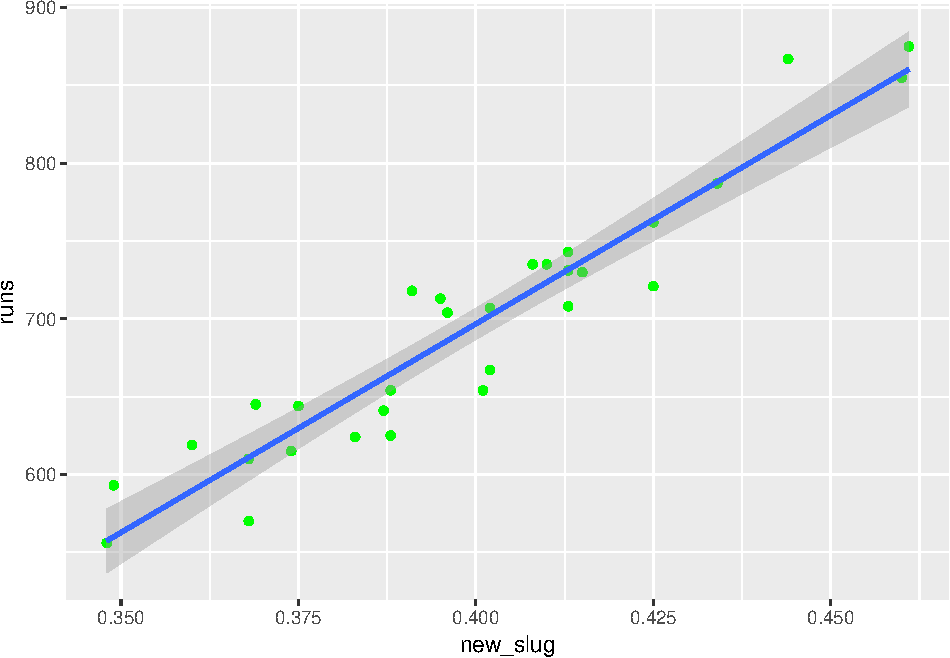
\includegraphics{DATA_606_Lab_7_files/figure-latex/unnamed-chunk-3-2.pdf}

\begin{Shaded}
\begin{Highlighting}[]
\KeywordTok{ggplot}\NormalTok{(mlb11, }\KeywordTok{aes}\NormalTok{(}\DataTypeTok{x=}\NormalTok{new_obs, }\DataTypeTok{y=}\NormalTok{runs)) }\OperatorTok{+}
\StringTok{  }\KeywordTok{geom_point}\NormalTok{(}\DataTypeTok{colour =} \StringTok{'green'}\NormalTok{) }\OperatorTok{+}
\StringTok{  }\KeywordTok{geom_smooth}\NormalTok{(}\DataTypeTok{method =} \StringTok{'lm'}\NormalTok{)}
\end{Highlighting}
\end{Shaded}

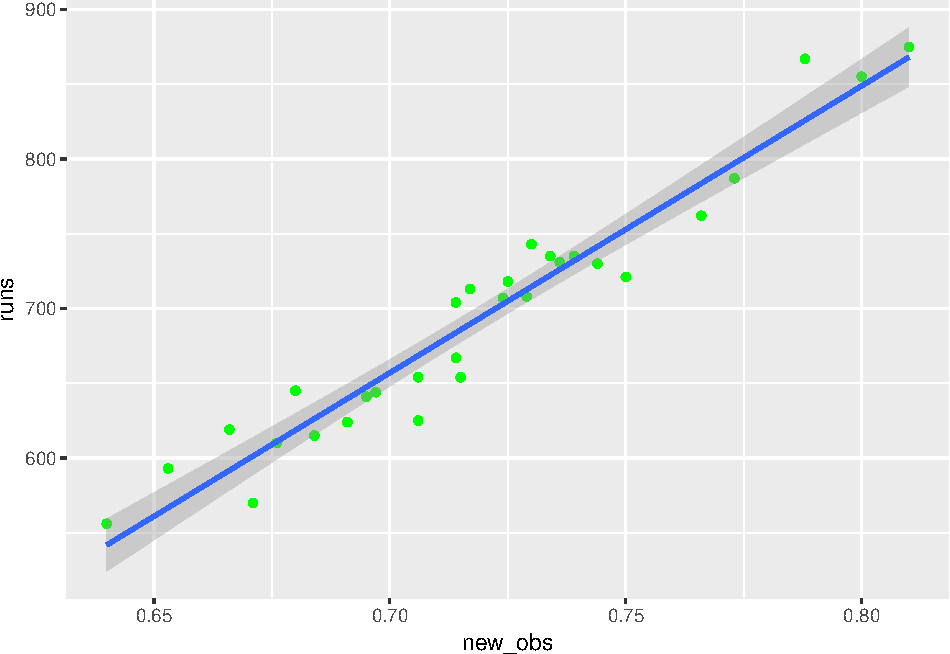
\includegraphics{DATA_606_Lab_7_files/figure-latex/unnamed-chunk-3-3.pdf}

\begin{Shaded}
\begin{Highlighting}[]
\NormalTok{m.}\DecValTok{1}\NormalTok{ <-}\StringTok{ }\KeywordTok{c}\NormalTok{(}\StringTok{'m8'}\NormalTok{, }\StringTok{'m9'}\NormalTok{, }\StringTok{'m10'}\NormalTok{)}
\NormalTok{r.squared.}\DecValTok{2}\NormalTok{ <-}\StringTok{ }\KeywordTok{c}\NormalTok{(}\KeywordTok{summary}\NormalTok{(m8)[[}\DecValTok{8}\NormalTok{]], }\KeywordTok{summary}\NormalTok{(m9)[[}\DecValTok{8}\NormalTok{]], }\KeywordTok{summary}\NormalTok{(m10)[[}\DecValTok{8}\NormalTok{]])}
\NormalTok{mdf.}\DecValTok{2}\NormalTok{ <-}\StringTok{ }\KeywordTok{data.frame}\NormalTok{(m.}\DecValTok{1}\NormalTok{, r.squared.}\DecValTok{2}\NormalTok{)}
\NormalTok{mdf.}\DecValTok{2}
\end{Highlighting}
\end{Shaded}

\begin{verbatim}
##   m.1 r.squared.2
## 1  m8   0.8491053
## 2  m9   0.8968704
## 3 m10   0.9349271
\end{verbatim}

\texttt{new\_obs} is the best predictor, which makes sense: number of
types getting a base hit, plus slugging efficiency would be a good
predictor.

\subsection{Question 13}\label{question-13}

Check the model diagnostics for the regression model with the variable
you decided was the best predictor for runs.

\subsubsection{Solution}\label{solution-12}

\begin{Shaded}
\begin{Highlighting}[]
\KeywordTok{par}\NormalTok{(}\DataTypeTok{mfrow =} \KeywordTok{c}\NormalTok{(}\DecValTok{1}\NormalTok{,}\DecValTok{2}\NormalTok{))}

\KeywordTok{hist}\NormalTok{(m10}\OperatorTok{$}\NormalTok{residuals)}

\KeywordTok{plot}\NormalTok{(m10}\OperatorTok{$}\NormalTok{residuals }\OperatorTok{~}\StringTok{ }\NormalTok{mlb11}\OperatorTok{$}\NormalTok{runs)}
\KeywordTok{abline}\NormalTok{(}\DataTypeTok{h =} \DecValTok{0}\NormalTok{, }\DataTypeTok{lty =} \DecValTok{3}\NormalTok{)}
\end{Highlighting}
\end{Shaded}

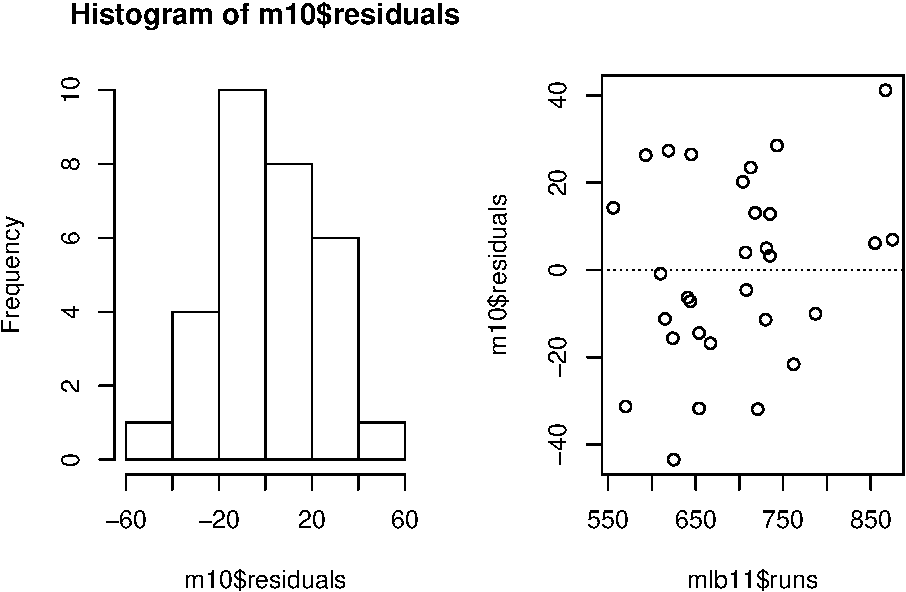
\includegraphics{DATA_606_Lab_7_files/figure-latex/unnamed-chunk-4-1.pdf}

\begin{Shaded}
\begin{Highlighting}[]
\KeywordTok{ggplot}\NormalTok{(mlb11, }\KeywordTok{aes}\NormalTok{(}\DataTypeTok{x=}\NormalTok{new_obs, }\DataTypeTok{y=}\NormalTok{runs)) }\OperatorTok{+}
\StringTok{  }\KeywordTok{geom_point}\NormalTok{(}\DataTypeTok{colour =} \StringTok{'green'}\NormalTok{) }\OperatorTok{+}
\StringTok{  }\KeywordTok{geom_smooth}\NormalTok{(}\DataTypeTok{method =} \StringTok{'lm'}\NormalTok{)}
\end{Highlighting}
\end{Shaded}

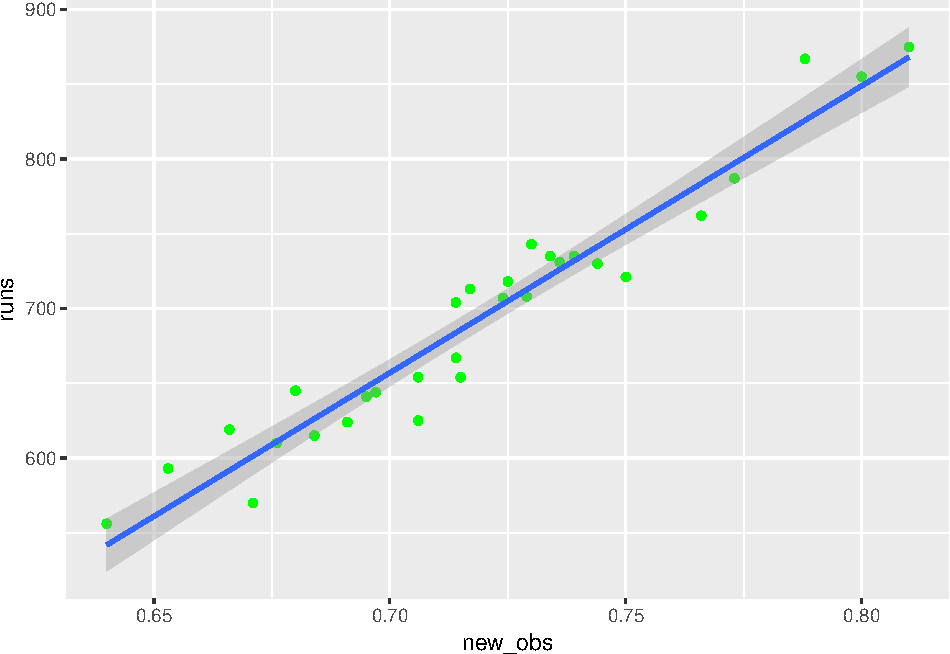
\includegraphics{DATA_606_Lab_7_files/figure-latex/unnamed-chunk-4-2.pdf}


\end{document}
